\documentclass[9pt]{beamer}

\usetheme{metropolis}
\usefonttheme[onlymath]{serif}

\usepackage{presentation}

\newcommand{\pp}{p\para}
\newcommand{\qp}{q\para}
\newcommand{\rp}{r\para}

\usepackage{fontspec}
\setsansfont{IBM Plex Serif}

\title{Interpretable Latent Variable Model for Molecular Design}
\subtitle{UGP Presentation}
\date{25th April, 2019}
\author{Gurpreet Singh}
\institute{Indian Institute of Technology, Kanpur}

\begin{document}
\frame{\titlepage}

\section{Background}

\subsection{Black Box Variational Inference}
\begin{frame}{BBVI - Overview}
	\begin{enumerate}
		\item[] <1-> In Variational Inference, the optimization objective is given by the ELBO
			\begin{align*}
				\logp{\pp{\vx}} \ge \elbo{\vx, \vphi} = \E[\vz \sim q(\vz \spipe \vx, \vphi)]{\logp{p(\vx, \vz)} - \logp{q(\vz \pipe \vx, \vphi)}}
			\end{align*}

		\item[] <2-> Black Box Variational Inference is based on stochastic optimization of the variational objective
			\begin{align*}
				\nabla \elbo{\vx, \vphi} &= \E[q(\vz \spipe \vx, \vphi)]{\nabla_\vphi \logp{q(\vz \pipe \vx, \phi)} \para{\logp{p(\vx, \vz)} - \logp{q(\vz \pipe \vx, \vphi)}}}
			\end{align*}

			The above term is known as the Score Function.
	\end{enumerate}

\end{frame}

\begin{frame}{BBVI - Reparameterization}
	\begin{enumerate}
		\item[] <1-> If we can find a reparametrization $\vepsilon = f^{-1}(\vz, \vphi)$ such that $\vepsilon$ is independent of $\vphi$, then
			\begin{align*}
				\nabla \elbo{\vx, \vphi} = \E[q(\vepsilon)]{\nabla_\vz \brac{\logp{p(\vx, \vz)} - \logp{q(\vz \pipe \vx, \vphi)}}_{\vz = f(\vepsilon, \vphi)} \nabla_{\vphi} f(\vepsilon, \vphi)}
			\end{align*}

		\item[] <2-> If $\vz$ is discrete $p(\vz)$ is a p.m.f. and therefore, the derivatives no longer exist. Hence, reparameterization is \bt{not} possible
	\end{enumerate}
\end{frame}

\begin{frame}{Discrete Latent Variables}
	Some methods to train discrete latent variable models -
	\begin{enumerate}
		\item Marginalize all discrete latent variables
		\item Using local expectation gradients, and reparametrization and marginalization % Essentially based on the idea that the value of a parameter depends only on a few values, however requires multiple function evaluations per gradient
		\item Relaxed computation of discrete densities (straight through approach)
		\item Smooth relaxations for discrete variables (e.g. Concrete Distribution)
		\item Using the Score Function approach with variance reduction using control variates/non-uniform sampling.
	\end{enumerate}
\end{frame}

\subsection{Gumbel-Softmax Trick}
\begin{frame}{The Concrete Distribution}
	Sampling from a categorical distribution: Sample U from a $\brac{0, 1}$ uniform distribution, then reparameterize as
	\begin{align*}
		\sC = \argmax{k \in \brac{K}} \logp{\alpha_k} - \log{-\log{\sU_k}}
	\end{align*}

	A softmax version of this can be used as smooth relaxations
	\begin{align*}
		\sZ_k = \frac{\texp{\para{\logp{\alpha_k} + G_k} / \tau}}{\sum_{k' = 1}^K \texp{\para{\logp{\alpha_{k'}} + G_{k'}} / \tau}}
	\end{align*}
	where $\tau$ is the \bt{temperature} parameter.
\end{frame}

\section{The Gumbolt Trick}
\begin{frame}{RBM Prior}
	Gumbel-Softmax trick only works for factorial priors. The Gumbolt trick offer an approach which allows us to work with more expressive priors, the (Restricted) Boltzmann Machine priors.

	\bt{Boltzmann Machine Prior}
	\begin{align*}
		\qp{\vz} &= \frac{\exp{-E(\vz)}}{Z_\theta}, \hspace{0.5cm} \mt{where}\\
		E(\vz) &= \trans{\vz} \vb + \trans{\vz} \sW \vz
	\end{align*}

	\bt{Restricted Boltzmann Machine Prior}
	\begin{align*}
		E(\vz) &= \trans{\vz_1} \vb_1 + \trans{\vz_2} \vb_2 + \trans{\vz_1} \sW \vz_2
	\end{align*}
\end{frame}
\begin{frame}{Gumbolt - Relaxed ELBO}
	\begin{enumerate}
		\item[] <1-> The posterior and the prior for the smoothing variables are given as
			\begin{align*}
				\pp{\vzeta \pipe \vtheta} &= \frac{\exp{-E_{\vtheta}(\vzeta)}}{\widetilde{Z}_{\vtheta}}, \ \mt{where} \widetilde{Z}_\vtheta = \int_\vzeta \exp{E_\vtheta(\vzeta)} \id \vzeta \\
				\qp{\vzeta \pipe \vx, \vphi} &= \prod_{i} \zeta_i q_i + (1 - \zeta_i)(1 - q_i)
			\end{align*}

		\item[] <2-> The alternate ELBO, therefore, is given as
			\begin{align*}
				\widetilde{\cL}\para{\vx, \vphi} = &\E[\qp{\vzeta \spipe \vx, \vphi}]{\logp{\pp{\vx \pipe \vzeta, \vtheta}} - \logp{\qp{\vzeta \pipe \vx, \vphi}} - E_\vtheta(\vzeta)} - \logp{\widetilde{Z}_{\vtheta}}
			\end{align*}
	\end{enumerate}
\end{frame}

\begin{frame}{Gumbolt - Relaxed ELBO}
	\begin{enumerate}
		\item[] <1-> Relaxed ELBO is given as
			\begin{align*}
				\breve{\cL}\para{\vx, \vphi} = &\E[\qp{\vzeta \spipe \vx, \vphi}]{\logp{\pp{\vx \pipe \vzeta, \vtheta}} - \logp{\qp{\vzeta \pipe \vx, \vphi}} - E_\vtheta(\vzeta)} - \logp{Z_{\vtheta}}
			\end{align*}

		\item[] <2-> We have
			\begin{align*}
				\logp{\pp{\vx \pipe \vtheta}} \ge \widetilde{\cL}\para{\vx, \vphi} \ge \breve{\cL}\para{\vx, \vphi}
			\end{align*}

		\item[] <3-> Also, as $\tau \ra 0$, $\breve{\cL} \ra \widetilde{\cL}$.

			Since as $\tau \ra 0$, we have $\vzeta \ra \vz$, therefore $\breve{\cL} \ra \widetilde{\cL} \ra \cL$
	\end{enumerate}
\end{frame}

\begin{frame}{Gumbolt - Regeneration}
	\begin{figure}[htpb]
		\centering
		\includegraphics[height=200px]{includes/plots/gumbolt-vae/mnist/regenerated.png}
		\caption{Regerenation Plot for Gumbolt-Vae}
	\end{figure}
\end{frame}

\begin{frame}{Gumbolt - Sampling}
	\begin{figure}[htpb]
		\centering
		\includegraphics[height=200px]{includes/plots/gumbolt-vae/mnist/sampled.png}
		\caption{Sampling Plot for Gumbolt-Vae}
	\end{figure}
\end{frame}

\section{Molecular Design}
\begin{frame}{Molecular Representations}
	\begin{enumerate}
		\item <1-> SMILES - offers a string representation of the molecule's skeletal structure
			\begin{figure}[htpb]
				\centering
				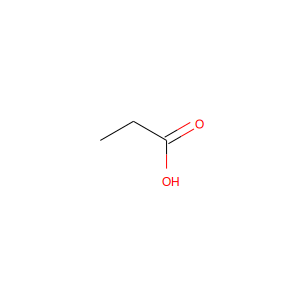
\includegraphics[height=50px]{includes/smiles-example.png}
			\end{figure}
			The SMILES string of the above molecule is given as ``CCC(=O)O''
		\item <2-> Molecular Graphs - assumes each atom to be a node and each bond to be an edge.
	\end{enumerate}
\end{frame}

\begin{frame}{Automatic Molecular Design}
	\begin{figure}[htpb]
		\centering
		\includegraphics[width=\textwidth]{includes/mol-design.png}
	\end{figure}
	Many deep learning based generative models have been proposed lately for automatic molecule design. Two common approaches are GANs and VAEs (our focus). Two categorizations -
	\begin{enumerate}
		\item SMILES based models
		\item Graph based model
	\end{enumerate}
\end{frame}

\begin{frame}{SMILES based models}
	\begin{enumerate}
		\item <1-> \bt{CVAE} -- Modifies vanilla VAEs to use convolutional layers in the encoder and layers of GRU networks for the decoder to predict sequences of strings (SMILES)
		\item <2-> \bt{GVAE} -- Improves upon CVAE by utilizing the parse trees (CFG) generated from SMILES strings as the molecular representaiton and using Grammar Variational Autoencoders as their architecture. Generates syntactically correct SMILES strings.
		\item <3-> \bt{SD-VAE} -- Incorporates semantics into the parse trees (Attribute Grammars) to generate syntactically as well as semmantically coherent SMILES strings.
	\end{enumerate}
\end{frame}

\begin{frame}{Problem with SMILES}
	\begin{figure}[htpb]
		\centering
		\includegraphics[width=\textwidth]{includes/smiles-problem.png}
	\end{figure}
\end{frame}

\begin{frame}{Molecular Graph based models}
	\begin{enumerate}
		\item <1-> \bt{VAE with Regularization Framework} -- Uses Variational Graph Autoencoders with additional constraints on graph connectivity and edge types
		\item <2-> \bt{CGVAE} -- Generates molecular graphs using sequential graph generation utilizing Gated Graph Neural Networks in both the encoder and the decoder.
			\vspace{1cm}
		\item[] <3-> \bt{Problem:} Invalid intermediate structures while sequential generation
	\end{enumerate}
\end{frame}

\begin{frame}{Junction Tree Variational Autoencoder (JT-VAE)}
	JT-VAE generates molecular graphs in two phases
	\begin{enumerate}
		\item <1-> It generates a tree-structured object (a junction tree) that  represents  the  scaffold  of subgraph  components and  their  coarse  relative  arrangements
		\item <2-> The subgraphs (nodes in the junction tree) are assembled into a coherent molecule graph using a graph message passing network. This approach incrementally generates the molecular graph while maintaining molecular validity at every step.
		\item[] <3-> \noindent{Thus, the JT-VAE encoder has two parts: graph encoder and tree encoder, so has the decoder: tree decoder and graph decoder. The graph and tree encoders are closely related to message passing neural networks (MPNNs)}
	\end{enumerate}
\end{frame}

\begin{frame}{JT-VAE (Continued)}
	\begin{itemize}
		\item <1-> The molecular structure is encoded into a two-part continuous latent representation $\vz = \para{\vz_\sT, \vz_\sG}$ where $\vz_\sT$ encodes the tree structure and what the subgraph components are in the tree. $\vz_\sG$ encodes the graph to capture the fine-grained connectivity
		\item <2-> Both the molecular graph and junction tree are encoded via message passing using adapted gated recurrent units (GRUs).
		\item <3-> The junction tree is sequentially generated with message passing in a top-down as well as bottom-up (Contains topological and label predictions)
		\item <4-> Graph decoding is performed in an alternating manner where a subgraph (for each node of the tree) is updated using messages generated by the tree encode
	\end{itemize}
\end{frame}

\section{Gumbolt JT-VAE}
\begin{frame}{Gumbolt Junction Tree VAE}
	Binary latent vectors ($\vb$) are used in company with real latent vectors ($\vr$), and the Gumbolt trick is employed to reparameterize the binary latent vectors (with RBM prior). Final latent representation $\vz$ is given as $\vz = \vb \odot \vr$
\end{frame}

\begin{frame}{Gumbolt JT-VAE: Architecture}
	\bt{The Decoder}
	\begin{align*}
		\brac{\vb_1, \vb_2} \sim \text{RBM}\para{\va_1, \va_2, \sW}, \hspace{0.5cm} \vr \sim \ND{\vzero, \vI}
	\end{align*}
	\bt{The Encoder}
	\begin{align*}
		\qp{\vb_n, \vr_n \pipe \vx, \sA, \vphi} &= \prod_{k = 1}^K \qp{b_{n,k} \pipe \vx_n, \sA, \vphi} \qp{r_{n,k} \pipe \vx_n, \vb_n, \sA, \vphi}
	\end{align*}
	and
	\begin{align*}
		\qp{b_{n, k} \pipe \vx, \sA, \vphi} &= \text{Bernoulli}\para{\pi_{n, k}} \\
		\qp{r_{n, k} \pipe \vx, \sA, \vphi} &= \ND{\mu_{n, k}, \sigma_{n, k}^2}
	\end{align*}
	where $\set{\pi_{n, k}}_{k = 1}^K = \tfunc{FC}{\vh_n}$, $\set{\mu_{n, k}, \sigma_{n, k}}_{k = 1}^K = \tfunc{FC}{\vh_n, \vb_n}$ and $\vh_n = \tfunc{MPNN}{\vx_n, \sA}$
\end{frame}

\begin{frame}{Comparison with JT-VAE (ZINC Dataset)}
	\fontsize{7.5pt}{7.2}\selectfont
	\begin{table}
		\centering
		\begin{tabular}{|c|c|}
			\hline
			\bt{Gumbolt JT-VAE} & \bt{JT-VAE} \\
			\hline
			3.889 & 4.019 \\
			\hline
		\end{tabular}
		\caption{Reconstruction Loss}
	\end{table}

	\fontsize{7.5pt}{7.2}\selectfont
	\begin{table}
		\centering
		\begin{tabular}{|l|c|c|}
			\hline
			& \bt{Gumbolt JT-VAE} & \bt{JT-VAE} \\
			\hline
			\bt{Topological Accuracy} & 93.38 & \bt{94.16} \\
			\hline
			\bt{Classification Accuracy} & \bt{99.21} & 97.57 \\
			\hline
			\bt{Assembly Accuracy} & \bt{95.34} & 94.31 \\
			\hline
		\end{tabular}
		\caption{Model Accuracies}
	\end{table}
\end{frame}

\begin{frame}{Qualitative Analysis - Neighborhood Sampling}
	\begin{figure}[htpb]
		\centering
		\includegraphics[width=\textwidth]{includes/plots/linear-local-samples.png}
	\end{figure}
\end{frame}

\begin{frame}{Qualitative Analysis - Sampling from the Prior}
	\begin{figure}[htpb]
		\centering
		\includegraphics[width=\textwidth]{includes/plots/plots.png}
	\end{figure}
\end{frame}

\begin{frame}{Further Possible Extensions}
	\begin{enumerate}
		\item Replace Teacher Forcing with Scheduled Sampling
		\item Avoid choosing a node as root in the Junction Tree
	\end{enumerate}
\end{frame}


\end{document}
